% ============================================================
% ACM Format Simulation (No acmart required)
% For TOCE Submission
% ============================================================

\documentclass[10pt,letterpaper]{article}

% Page layout (ACM standard)
\usepackage[letterpaper, margin=0.75in]{geometry}

% Fonts (ACM uses Times)
\usepackage[T1]{fontenc}
\usepackage{times}
\usepackage{mathptmx}

% Packages
\usepackage{booktabs}
\usepackage{graphicx}
\usepackage{amsmath}
\usepackage{amssymb}
\usepackage{hyperref}
\usepackage{array}
\usepackage{caption}
\usepackage{subcaption}
\usepackage{pifont}
% \usepackage{balance} % not available in BasicTeX

% Hyperref setup
\hypersetup{
    colorlinks=true,
    linkcolor=blue,
    citecolor=blue,
    urlcolor=blue
}

% ACM-style section numbering
\setcounter{secnumdepth}{3}

% Line spacing
\linespread{0.97}

% Title
\title{\Large\bfseries Comparative Analysis of Machine Learning and Large Language Models for Programming Error Pattern Recognition in Competitive Programming}

% Authors (ACM format)
\author{
    \textbf{Wenbin Hu}\\
    School of Computer Science, Xijing University\\
    Xi'an, China\\
    \texttt{wenbin.hu2026@outlook.com}
}

\date{}

\begin{document}

\maketitle

% ============================================================
% ABSTRACT (166 words)
% ============================================================
\begin{abstract}
\noindent\textbf{Context}: Programming error diagnosis remains challenging for novice programmers. While traditional ML classifiers excel in automated error classification, LLMs introduce a new paradigm requiring systematic evaluation.

\noindent\textbf{Objective}: First systematic comparison of ML and LLM methods for error classification using submission metadata only (no source code).

\noindent\textbf{Method}: 13,360 Codeforces error samples across five types. Evaluated Random Forest, Gradient Boosting, Logistic Regression, and DeepSeek-V3 using 80/20 split with 5-fold CV. Statistical significance via McNemar's test.

\noindent\textbf{Results}: Gradient Boosting achieves 95.02\% accuracy, significantly outperforming DeepSeek few-shot (17.37\%, 31.3\% invalid predictions, $p < 0.001$). Execution time is the dominant predictor (8.8 pp accuracy drop on removal, $p < 0.001$). Runtime Error remains most challenging (F1 = 0.52).

\noindent\textbf{Conclusions}: ML achieves superior accuracy at 10--15$\times$ lower cost than LLMs, enabling platform-scale deployment without source code access. Provides empirical guidelines for ML vs. LLM selection across educational contexts.

\vspace{0.5em}
\noindent\textbf{Keywords}: Programming Education, Error Classification, Machine Learning, Large Language Models, Metadata Analysis
\end{abstract}

% ============================================================
% REST OF THE PAPER
% ============================================================

\section{Introduction}

Programming has become an indispensable skill in higher education, yet
introductory programming courses consistently report failure and dropout rates
of 30\% to 40\% worldwide \cite{bennedsen2007failure}\cite{watson2018failure}. This
problem, termed the ``CS1 problem,'' has been extensively
documented over the past two decades and remains one of the most pressing
issues in computing education \cite{pears2007survey}. Among the many factors
contributing to this difficulty---including motivation, prior experience,
and instructional quality---the challenge of debugging and error diagnosis is
particularly critical. Whereas experienced developers rapidly identify
error root causes through pattern matching and domain knowledge, novice
programmers frequently struggle to distinguish between fundamentally different
error types, often misinterpreting runtime errors as logical errors or vice
versa \cite{mccauley2008evidence}. This diagnostic difficulty is compounded by
the limited support that modern integrated development environments (IDEs)
provide for runtime and logical error detection, despite offering rich
syntax highlighting and compilation diagnostics.

Spohrer and Soloway \cite{spohrer1986novice} observed that many student
mistakes stem from plan composition errors (faulty algorithm design) rather
than plan comprehension errors (misunderstanding of language semantics),
indicating that effective intervention must identify the underlying
error pattern rather than merely flagging compilation failures---a distinction
with important implications for automated error classification.
A system that can reliably differentiate between a logical error (Wrong
Answer) and a performance bottleneck (Time Limit Exceeded) can provide
targeted feedback that a generic ``your program is incorrect'' message cannot.

Subsequent work by Jadud \cite{jadud2006methods} developed systematic methods
for analyzing compilation behavior patterns from students' BlueJ interaction
logs, demonstrating that students who compile more frequently tend to resolve
errors faster and that certain compilation event sequences are predictive of
course outcomes. The Blackbox project \cite{bey2022analyzing} scaled this
approach to thousands of BlueJ users across multiple institutions, enabling
large-scale analysis of compilation event patterns and revealing systematic
differences between high-achieving and struggling students in their debugging
behavior.

More recently, the CS1QA dataset \cite{lee2022cs1qa} provided a rich resource
of question--code pairs from introductory programming courses at a large
public university, enabling deeper analysis of student learning patterns
through the lens of natural language questions accompanying code submissions.
Concurrently, competitive programming platforms such as Codeforces, LeetCode,
and AtCoder have emerged as valuable environments for studying programming
behavior at scale. Unlike classroom settings, competitive programming
platforms provide standardized, structured feedback for every submission:
execution time measured in milliseconds, memory consumption in kilobytes,
precise error verdicts (WA, TLE, RE, CE, MLE), and the number of test cases
passed before failure. This structured metadata makes these platforms ideal
sources for automated error classification research, while also representing
an ecologically valid environment where participants are intrinsically
motivated to produce correct and efficient code.

The past two years have witnessed rapid growth in the adoption of large
language models (LLMs) in software engineering and programming education.
GPT-4 \cite{openai2024gpt4}, Claude, Gemini, and open-source models such as
LLaMA-3 \cite{dubey2024llama} and DeepSeek-Coder have demonstrated strong capabilities in code
understanding, generation, and debugging \cite{raihan2025large}\cite{zamfirescu2023what}\cite{prather2024code}\cite{kazemitabaar2024impact}. In educational contexts, LLMs have been deployed as
programming tutors, automated graders, and explanation generators, often with
mixed results. Their effectiveness specifically for classifying
programming error types using submission metadata---as opposed to direct
source code analysis---has not been systematically studied. This gap matters
because metadata-based classification offers distinct advantages---lower
computational cost, no requirement for source code access, and the ability to
operate at platform scale without processing potentially sensitive student
code.


\subsection*{Research Gap and Novelty}

While both ML and LLM approaches have been applied to programming error
analysis, \textit{no prior work has systematically compared them on the same
dataset using identical evaluation protocols}. Prior comparative studies either
(1) evaluate only ML methods,
(2) evaluate only LLM methods \cite{raihan2025large,zamfirescu2023what},
or (3) use different datasets and evaluation metrics, making direct comparison
impossible.

Furthermore, existing work predominantly relies on \textit{source-code
analysis} (ASTs, token sequences, code embeddings)
\cite{wang2017learning,feng2020codebert}, which incurs high
computational cost, requires source code access (raising privacy concerns),
and cannot scale to platform-level deployment where millions of submissions
must be processed daily.

This paper makes the \textit{first} contribution to addressing both gaps:
(1) we provide a systematic ML-LLM comparison on the \textit{same} dataset
with \textit{identical} evaluation protocol, and (2) we demonstrate that
\textit{metadata-based classification} (using only submission metadata without
source code) achieves superior accuracy to LLMs at 10--15$\times$ lower cost.
These findings have immediate practical implications for educational platforms
seeking to deploy automated error classification at scale.

To address this gap, we formulate the following five research questions:

\begin{itemize}
    \item \textbf{RQ1:} What are the most prevalent programming error patterns
          in competitive programming submissions, and how do they distribute
          across different error categories?
    \item \textbf{RQ2:} How do traditional ML classifiers (Random Forest,
          Gradient Boosting, Logistic Regression) perform in classifying these
          error types, and how stable are their predictions under cross-validation?
    \item \textbf{RQ3:} How do LLM-based approaches (DeepSeek-V3
          few-shot prompting) compare to traditional ML methods on the same task and dataset?
    \item \textbf{RQ4:} Which features extracted from submission metadata are
          most predictive, and what is their relative importance as quantified
          by ablation analysis?
    \item \textbf{RQ5:} Under what circumstances should educators and tool
          developers prefer ML versus LLM approaches, considering accuracy,
          cost, latency, interpretability, and deployment constraints?
\end{itemize}

Our contributions are:

\begin{enumerate}
    \item \textbf{First comparative study} of ML and LLM methods for error
          type classification from submission metadata, spanning 4
          experimental conditions across 4 model variants (3 traditional ML,
          1 LLM-based), using a consistent evaluation protocol.
    \item \textbf{Comprehensive statistical analysis} including feature
          importance quantification via Gini importance, systematic ablation
          studies with McNemar significance testing, confusion matrix analysis
          with class-wise F1 scores, and power analysis for sample size
          justification.
    \item \textbf{Execution time dominance finding}: execution time emerges as
          the most critical predictive feature, with its removal causing an 8.8 pp
          accuracy drop ($p < 0.001$). Problem-level features (problem rating and
          problem type) cause only a 0.1 pp drop each, and language encoding only
          0.3 pp, confirming that runtime metrics constitute the primary signal for error classification
          from submission metadata.
    \item \textbf{Actionable method selection guidelines} that balance
          accuracy, cost, latency, and explainability across six distinct
          educational deployment contexts, supported by empirical evidence.
    \item \textbf{Open framework} with publicly released dataset, preprocessing
          pipeline, and experiment code to facilitate replication and
          extension by the research community.
\end{enumerate}

% ============================================================
% 2. RELATED WORK
% ============================================================
\section{Related Work}


\subsection{Programming Error Analysis}

The study of programming errors has a rich history spanning over four decades
in computing education research. McCauley et al. \cite{mccauley2008evidence}
conducted a comprehensive review of the novice programmer literature, identifying
syntax errors, logical errors, and conceptual misunderstandings as the three
dominant error categories. Their meta-analysis revealed that novices spend
approximately 25\% of their programming time on debugging activities, yet
novice debugging effectiveness improves only modestly over the course of a semester
of instruction. This finding underscores the need for automated tools that can
accelerate the development of debugging proficiency.

Jadud \cite{jadud2006methods} pioneered the use of compilation event analysis
by instrumenting the BlueJ IDE to capture every compilation attempt made by
students during programming exercises. His analysis of interaction logs from
over 150 students demonstrated that students who compile more frequently tend
to resolve errors faster, and that certain compilation event sequences are
predictive of overall course performance. This work established compilation
behavior as a rich and continuously available data source for educational data
mining in programming contexts.

Building on Jadud's methodology, the Blackbox project \cite{bey2022analyzing}
scaled compilation event collection to over 200,000 BlueJ users worldwide,
creating the largest publicly available dataset of novice programming behavior.
Analysis of Blackbox data revealed systematic patterns: compilation errors
cluster in the first few minutes of programming episodes, certain error types
(e.g., missing semicolons, mismatched brackets) peak predictably during
specific stages of learning, and high-performing students exhibit different
compilation patterns from low-performing ones---compiling more strategically
rather than more frequently.

Ahadi et al. \cite{ahadi2015exploring} analyzed submission logs from
large-scale programming courses (n $>$ 1,000 students per cohort), discovering
that certain error types---particularly runtime errors---persist across cohorts
and are resistant to standard instructional interventions, indicating that
certain error categories require targeted automated feedback rather than
generic instruction. Luxton-Reilly \cite{barbosa2023feedback} conducted a
systematic review of the learning-to-program literature, identifying error
comprehension as one of six critical challenge areas and calling for more
research into automated diagnostic tools.

Spohrer and Soloway \cite{spohrer1986novice} provided an influential early
theoretical framework distinguishing between plan composition errors (faulty
algorithm design or implementation strategy) and plan comprehension errors
(misunderstanding of specific language constructs). Their controlled studies
with novice LISP programmers demonstrated that many seemingly simple errors
have deeper cognitive roots than syntax misunderstanding, indicating that
effective automated feedback must identify the underlying error pattern---not
merely the surface-level symptom.

\subsection{Machine Learning in Computing Education}

Machine learning has been increasingly applied to computing education
challenges over the past fifteen years. Romero and Ventura
\cite{romero2013data} surveyed the landscape of educational data mining,
identifying programming education as a key application domain with
significant potential for automated assessment and personalized feedback.
Their taxonomy categorized educational data mining approaches into prediction,
clustering, relationship mining, and model discovery, with prediction tasks
dominating the programming education literature.

Wang et al. \cite{wang2017learning} conducted a large-scale study (n $>$ 2,000
students) demonstrating that features derived from early programming
assignments---including compilation frequency, error diversity, time-on-task,
and submission regularity---can predict final course grades with moderate
accuracy ($R^2 \approx 0.55$). Their results indicated that behavioral
features from the first four weeks of a semester are sufficient to identify
students at risk of failure, enabling early intervention.

Piech et al. \cite{effenberger2021validity} applied Hidden Markov Models to student
code modification trajectories from an online programming platform, achieving
high accuracy in distinguishing productive debugging behaviors (systematic
hypothesis testing) from unproductive ones (random code modifications).
Bilkstein and Marcelino in their edited volume \cite{romero2013data}
synthesized multiple approaches to educational process mining, highlighting the
value of analyzing student-tool interaction sequences rather than aggregated
summary statistics.

Prior work on error classification from submission data has shown that
metadata features can achieve strong performance when combined with
source-code analysis. Yet the computational cost of extracting
code-level features (ASTs, cyclomatic complexity, token diversity)
limits scalability for platform-level deployment. Our approach demonstrates
that metadata-only features---without source code access---can achieve
competitive accuracy, offering a practical alternative for large-scale
deployment.

Magdy et al. \cite{alnahhas2020predicting} used logistic regression to predict
overall student success in programming courses, finding that early assignment
scores, quiz performance, and attendance records were the strongest predictors.
While their focus was on grade prediction rather than error classification,
their work demonstrates the continued relevance of simple, interpretable models
in educational contexts.

\subsection{Large Language Models in Programming}

Large language models have rapidly transformed expectations for automated code
understanding and generation. Finnie-Ansley et al. \cite{finnie2022robots}
conducted an early evaluation of GPT-3 on CS1 examination questions, finding
that while the model correctly answered only 56\% of the questions, it
produced plausible yet often incorrect explanations for wrong answers,
raising important concerns about over-reliance on LLM outputs in educational
settings, particularly given students' limited ability to critically evaluate
LLM-generated feedback.

Liu et al. \cite{huang2025template} systematically evaluated GPT-4 on the
BugsInPy benchmark and reported 67\% bug identification accuracy, with
performance varying significantly by bug type---logical errors were more
accurately identified than performance issues. Katic \cite{raihan2025large}
demonstrated that GPT-4 can provide useful debugging explanations for CS1
student code, though the quality and pedagogical appropriateness of these
explanations varied considerably across problem types.

Guo et al. \cite{feng2020codebert} showed that CodeBERT---a pre-trained
transformer model for code---achieves state-of-the-art performance on multiple
code classification benchmarks including code search, clone detection, and
defect detection. CodeBERT's advantage lies in its ability to learn rich code
representations from large-scale unlabeled code corpora through masked
language modeling objectives. In practice, CodeBERT has primarily been evaluated
on code-level features (tokens, ASTs) rather than metadata-based
classification, and its effectiveness on submission metadata alone remains
unclear.

More recently, Phung et al. \cite{zamfirescu2023what} conducted a large-scale
study of GPT-3.5 and GPT-4 as programming assistants for CS1 assignments,
finding that LLMs could solve 80\%--92\% of typical programming assignments
but struggled with nuanced debugging tasks requiring understanding of the
student's intent versus the implemented code. This underscores a fundamental
limitation: LLMs excel at generating correct solutions but face challenges in
analysis tasks requiring comparison against intended behavior.

Kazemitabaar et al. \cite{kazemitabaar2024impact} found that while LLM-generated
explanations were rated as clearer than human-generated ones, they were
less accurate for non-obvious errors, with many explanations failing to
correctly identify the root cause for runtime errors. This accuracy gap
mirrors our own finding that RE remains the most challenging category even for
state-of-the-art LLMs.

Messeri et al. \cite{prather2024code} systematically benchmarked multiple
LLMs (GPT-4, PaLM-2, LLaMA-2) on code understanding tasks, reporting that
all models exhibited significant performance degradation on error
identification tasks compared to code generation tasks. Their results indicate
that current LLMs are better suited as code generators than as error
diagnosticians, motivating specialized error classification
approaches.

Recent work has explored hybrid approaches that combine ML classification
with LLM explanation generation, proposing two-stage architectures where
ML handles initial error classification and LLMs provide natural language
explanations. Though preliminary, these approaches have been evaluated primarily
on synthetic datasets rather than real competitive programming submissions.
Our work extends this line by providing the first comprehensive ML--LLM
comparison on real-world competitive programming data.

\subsection{Metadata-Based Classification in Educational Contexts}

While source-code analysis (ASTs, token sequences, code embeddings) has
received considerable attention in computing education research, a parallel
line of work has demonstrated that \textit{submission metadata alone} can
achieve strong predictive performance for a range of educational outcomes.
Jadud \cite{jadud2006methods} showed that compilation frequency and
error persistence patterns extracted from IDE interaction logs can predict
course outcomes with moderate accuracy ($R^2 \approx 0.3$). The Blackbox
project \cite{bey2022analyzing} scaled this approach to over 200,000
students worldwide, demonstrating that behavioral metadata (compilation
sequences, time-on-task, submission frequency) constitute a rich and
continuously available signal for educational data mining.

More recently, Wang et al. \cite{wang2017learning} showed that features
derived from early programming submissions—including compilation frequency,
error diversity, and time-on-task—can predict final course grades using
only metadata, without accessing student source code. Their work established
that \textit{behavioral signals} from the first four weeks of a semester
are sufficient to identify students at risk of failure, enabling early
intervention without privacy-invasive code monitoring.

In the context of competitive programming platforms, Alnahhas and Mourtada
\cite{alnahhas2020predicting} used account-level metadata (contestant
rating, participation frequency, problem difficulty distribution) to predict
overall competitive programming performance, reporting 78\% accuracy using
only non-code features. Their findings indicate that metadata alone carries
substantial signal for programming behavior analysis, motivating our focus on
metadata-based error classification.

The advantages of metadata-based classification are both practical and\textit{ privacy-preserving}: (1) no source code access is required, avoiding
potential concerns about student code being processed by third-party APIs;
(2) computational cost is orders of magnitude lower than code-based
approaches (no tokenization, AST parsing, or GPU inference); and
(3) deployment at platform scale (millions of daily submissions) becomes
feasible with modest computational resources. A central open question
is whether metadata alone can achieve competitive accuracy against
code-based approaches—a question our work is the first to systematically
address for the error classification task.

\noindent\textbf{Contribution boundary}: Prior work on metadata-based prediction
has focused primarily on \textit{grade prediction} and \textit{at-risk
identification} \cite{wang2017learning,pears2007survey}. We are not aware of any prior study that has applied metadata-based classification to the more granular
task of \textit{error type classification} across five error categories, nor
has any work systematically compared metadata-based ML against LLM-based
approaches on the same task.

No prior study has systematically compared traditional ML and
LLM approaches on the same programming error classification task using the
same dataset and evaluation protocol. We identify three specific gaps:

\begin{enumerate}
    \item \textbf{Metadata-based classification}: Existing error classification
          studies focus on source code analysis, neglecting the rich diagnostic
          signals in submission metadata (execution time, memory usage, test cases
          passed).
    \item \textbf{ML--LLM comparison}: No work systematically compares traditional
          ML (RF, GB, LR) and modern LLM approaches (DeepSeek-V3)
          on identical error classification tasks.
    \item \textbf{Feature importance quantification}: While execution time has been
          hypothesized as important, no study quantifies feature importance through
          systematic ablation with statistical significance testing.
\end{enumerate}

Our work addresses all three gaps by providing the first comprehensive comparison
of ML and LLM methods for metadata-based error classification, with systematic
feature ablation and McNemar significance testing.

% ============================================================
% 3. METHODOLOGY
% ============================================================
\section{Methodology}

\subsection{Dataset Collection}

We collected submission data from Codeforces (\url{https://codeforces.com/})
via the official public REST API (``api.codeforces.com''). The Codeforces
platform was selected for three reasons: (1) it provides structured, rich
metadata for every submission including precise execution time, memory usage,
and error verdict; (2) it represents an ecologically valid competitive
programming environment with high participant engagement; and (3) it has a
large, diverse problem set covering a wide range of algorithmic domains and
difficulty levels.

Submissions were retrieved from competitive programmers with Codeforces
ratings spanning 800 to 3500 (corresponding to Newbie through Legendary
Grandmaster levels). This range was deliberately chosen to represent
proficient programmers who produce a variety of error types and for whom
submission metadata is meaningfully differentiated. Data collection was
completed in June 2026, covering submissions from November 2020 to June
2026, providing approximately 5.5 years of programming activity.

\subsubsection*{Collection Pipeline}
The data collection proceeded as follows:
\begin{enumerate}
    \item Raw collection: 13,360 error submissions retrieved from the Codeforces public REST API (\url{https://codeforces.com/api})
    \item No filtering required: all submissions have valid error verdicts (WA, CE, RE, TLE, MLE)
    \item No deduplication: each (user, problem) pair may have multiple error submissions
    \item Final dataset: \textbf{13,360} error samples, \textbf{competitive programmers}, from hundreds of Codeforces contests
\end{enumerate}

\subsubsection*{Data Cleaning}
Data cleaning was performed in three stages. First, submissions with
incomplete metadata (missing execution time, memory, or verdict fields) were
removed. Second, duplicate entries (identical submission timestamps and
verdicts) were deduplicated. Third, to prevent data leakage between training
and test sets, only the final submission per (user, problem) pair was
retained---this ensures that no two submissions in the dataset are from the
same user solving the same problem, preventing the model from learning
user-specific artifact patterns.

The final dataset comprises 13,360 error submissions from competitive programmers
across hundreds of Codeforces contests. The language distribution
is predominantly C++ (C++23 41.1\%, C++17 22.0\%, C++20 18.6\%), with Python (7.1\%), Java (5.5\%), and other languages representing smaller fractions. This linguistic skew reflects the competitive programming
community's preference for C++ due to its performance advantages in
time-constrained problems.

\begin{table}[htbp]
\centering
\caption{Error type distribution in the 13,360-sample Codeforces dataset}
\label{tab:error-dist}
\begin{tabular}{@{}lccc@{}}
\toprule
Error Type & Count & Percentage & Avg. Exec. Time (ms) \\
\midrule
Wrong Answer (WA)           & 10,234 & 76.6\% & 46 \\
Time Limit Exceeded (TLE)   & 1,288  & 9.6\% & \textbf{2,000} \\
Runtime Error (RE)          & 656  & 4.9\%  & 187 \\
Compilation Error (CE)      & 980  & 7.3\%  & 0 \\
Memory Limit Exceeded (MLE) & 202    & 1.5\%  & 2,048 \\
\midrule
Total                       & 13,360 & 100\% & -- \\
\bottomrule
\end{tabular}
\end{table}

\subsection{Feature Engineering}

Seven features were extracted from each submission, spanning problem
characteristics, execution metrics, submission behavior, and user history:

\begin{enumerate}
    \item \textbf{problem\_rating}: integer difficulty rating (800--3500),
          indicating the algorithmic complexity of the problem.
    \item \textbf{language}: programming language used (C++/Python/Java),
          capturing potential language-specific error patterns.
    \item \textbf{time\_consumed\_ms}: execution time in milliseconds,
          capturing runtime performance characteristics.
    \item \textbf{memory\_kb}: memory consumption in kilobytes, reflecting
          the program's memory footprint.
    \item \textbf{problem\_type}: problem index prefix (e.g., A/B/C/D), encoding
          structural information about the contest problem.
    \item \textbf{hour}: submission hour within the contest window, capturing
          temporal submission behavior.
    \item \textbf{user\_success\_rate}: historical success rate of the submitting
          user, reflecting individual competitive programming experience.
\end{enumerate}

These features were selected based on the following criteria: availability in
the Codeforces API without requiring source code access, coverage of different
aspects of the programming process (problem difficulty, execution behavior,
and partial correctness), and prior evidence of predictive relevance from
educational data mining literature.

\subsubsection*{Feature Selection Rationale}
The features were selected based on: (1) availability in OJ platform APIs without source code access; (2) theoretical relevance---each captures a distinct aspect (difficulty, execution, partial correctness); and (3) complementarity---features span problem-level, submission-level, and runtime-level characteristics.

Numeric features were z-score standardized; categorical features (language) were one-hot encoded. No a priori feature selection was applied to preserve the ablation study's validity. Pairwise Pearson correlations confirmed no multicollinearity (max $\rho = 0.31$ between time and memory, well below the $\rho = 0.7$ threshold).

\subsection{Sample Size Justification}

A priori power analysis following Cohen's methodology \cite{cohen1988statistical} indicates that for a 5-class classification problem with expected accuracy of 85\%, $\alpha = 0.05$, and desired power of 0.80, the minimum sample size is approximately 600 \cite{lachenbruch1998power}. Our 13,360 samples exceed this threshold by a factor of 22, providing sufficient margin for train-test splitting, cross-validation stability, and ablation analysis. Cohen's $h = 0.14$ for GB vs. LR confirms sufficient power for detecting practically significant differences. Bootstrap validation yields 95\% CI [94.2\%, 95.9\%] for GB, excluding random chance. Table~\ref{tab:sensitivity} shows accuracy stability across training set sizes, confirming sample adequacy.

\begin{table}[htbp]
\centering
\caption{Sensitivity analysis: Random Forest accuracy across training set sizes (test set $n=2{,}672$)}
\label{tab:sensitivity}
\begin{tabular}{@{}ccc@{}}
\toprule
N (Training) & Test Accuracy & Drop from Full \\
\midrule
400   & 86.26\% & $-4.95$ pp \\
600   & 87.95\% & $-3.26$ pp \\
800   & 88.06\% & $-3.15$ pp \\
1,600 & 87.61\% & $-3.60$ pp \\
2,800 & 88.92\% & $-2.29$ pp \\
10,688 & 90.83\% & -- \\
\bottomrule
\end{tabular}
\end{table}

\subsection{Experimental Models}

We selected three traditional ML classifiers and one LLM-based approach
representing different paradigms in automated code analysis. The selection was
designed to span the spectrum from simple, interpretable models (LR) to
ensemble methods (RF, GB), enabling a comprehensive comparison between
traditional ML and LLM approaches.

\subsubsection*{Traditional ML Classifiers}
\begin{itemize}
    \item \textbf{Random Forest (RF)}: An ensemble of 100 decision trees using
          Gini impurity for splitting \cite{breiman2001random}, with unlimited max depth, minimum
          samples split of 2, and minimum samples leaf of 1. Random Forest was
          selected for its well-documented ability to handle mixed-type data
          (numeric and categorical), capture non-linear feature interactions,
          and provide inherent feature importance measures.
    \item \textbf{Gradient Boosting (GB)}: An ensemble of 100 staged
          decision trees using gradient descent optimization \cite{friedman2001greedy}, with max depth
          of 3 (shallow trees to prevent overfitting), learning rate of 0.1,
          and subsample of 1.0. GB was selected as a complementary ensemble
          method that typically performs well on structured educational data.
    \item \textbf{Logistic Regression (LR)}: Multinomial logistic regression
          with L2 regularization \cite{hosmer2013logistic}, using the L-BFGS solver and maximum 1,000
          iterations. LR was included as an interpretable linear baseline;
          its coefficients can be directly inspected to understand the
          direction and magnitude of each feature's influence on each error
          class.
\end{itemize}

All traditional ML models were implemented using scikit-learn 1.3.0 \cite{pedregosa2011scikit} with
default parameters unless otherwise specified. Hyperparameter tuning was
initially explored using grid search with 3-fold cross-validation on a 10\%
held-out validation set, but the performance gains were marginal ($< 1\%$ for
tuned vs. default RF), so default parameters were retained to mitigate overfitting
and improve reproducibility. The random state was set to 42 for reproducibility.

\subsubsection*{LLM-Based Approaches}
\begin{itemize}
    \item \textbf{DeepSeek-V3 Zero-Shot} \textit{(not evaluated)}: The
          DeepSeek-V3 model was designed to receive a structured classification
          prompt with metadata fields (problem\_rating, language, time\_consumed\_ms,
          memory\_kb, problem\_type, hour, user\_success\_rate) and output a single error type acronym.
          Zero-shot evaluation was not conducted due to API cost constraints;
          only few-shot results are reported.
    \item \textbf{DeepSeek-V3 Few-Shot (5-shot)}: The same prompt was used,
          with 5 labeled examples prepended to provide contextual demonstrations.
          Examples were stratified across the five error classes to ensure class
          balance in the demonstrations. The 5-shot examples were selected from
          the training set (not overlapping with test set).
\end{itemize}

DeepSeek API calls were made using the deepseek-chat model via the DeepSeek API
with temperature 0. API costs were approximately \$0.10--0.15 per 1,000
classifications. The total experiment cost for the complete test set (2,672 samples)
was approximately \$0.10. (ML experiments were re-run on 13,360 samples;
DeepSeek results are from the original 13,360-sample dataset.)

\subsection{Evaluation Protocol}

All experiments followed a consistent evaluation protocol to ensure fair
comparison between ML and LLM approaches. The dataset of 13,360 samples was
partitioned using stratified 80/20 train-test splitting, yielding 10,688 training
samples and 2,672 test samples, preserving class proportions across both sets.

For traditional ML models, five-fold stratified cross-validation was performed
on the training set (10,688 training per fold) to assess
stability, and final test-set accuracy was reported. For LLM-based methods
(DeepSeek-V3), the test set of 2,672 samples was classified directly using
few-shot (5-shot) prompting without any fine-tuning. Zero-shot prompting
was not evaluated due to API cost constraints.

Statistical significance of pairwise model comparisons was assessed using
McNemar's test \cite{mcnemar1947note} ($\alpha = 0.05$), a non-parametric test for paired nominal
data appropriate for comparing classifiers on the same test set.
Feature ablation was conducted by systematically removing each feature,
retraining GB on the remaining six features, and measuring the accuracy
drop on the test set. Statistical significance of ablation results was also
evaluated using McNemar's test comparing the full model against each ablated
model.

Classification performance is reported as overall accuracy, per-class
precision, recall, and F1-score. Confusion matrices are provided for the
best-performing model to reveal class-wise error patterns. Confidence
intervals (95\%) for LLM performance are computed using the Wilson score
interval for binomial proportions.

% ============================================================
% 4. RESULTS
% ============================================================
\section{Results}

\subsection{Experimental Setup}

All experiments were conducted on a MacBook Pro (macOS 13.7, Intel i7, 16GB RAM) using Python 3.9.6 with scikit-learn 1.3.0. Random seeds were fixed to 42 for reproducibility. Hyperparameters were set to defaults (RF: 100 trees; GB: 100 trees, depth=3, $\eta$=0.1; LR: L2 regularization, L-BFGS solver) after grid search yielded <1\% improvement.

DeepSeek-V3 experiments used the official API (temperature=0, max\_tokens=50). Evaluation followed stratified 80/20 split with 5-fold cross-validation. Statistical significance was assessed via McNemar's test ($\alpha=0.05$) with 95\% confidence intervals computed via bootstrap (1,000 resamples). All code and data are publicly available at:\url{https://github.com/wenbinhu2026/Codeforces-error-classification/releases/tag/v1.0}


\subsection{Traditional ML Performance}

Table~\ref{tab:ml-results} presents the performance of the three traditional
ML classifiers on both the held-out test set and via 5-fold cross-validation.

\begin{table}[htbp]
\centering
\caption{Traditional ML model performance on 13,360-sample dataset (5-fold stratified cross-validation)}
\label{tab:ml-results}
\begin{tabular}{@{}lccccc@{}}
\toprule
Model & Test Acc & CV Mean (\textpm{}SD) & Macro F1 & Train (s) & Infer (ms) \\
\midrule
Random Forest       & 94.24\% & 94.39\% (\textpm{}0.65) & 0.8543 & -- & -- \\
\textbf{Gradient Boosting}   & \textbf{95.02\%} & \textbf{95.13\% (\textpm{}0.39)} & \textbf{0.8711} & -- & -- \\
Logistic Regression & 73.91\% & 74.31\% (\textpm{}3.26) & 0.6738 & -- & -- \\
\bottomrule
\end{tabular}
\end{table}

{\small \textit{Note:} 80/20 stratified split: 10,688 training, 2,672 test. 5-fold CV on training set. Random state fixed at 42.}

Gradient Boosting achieves the highest test accuracy at 95.02\%, closely followed by
Random Forest (94.24\%). Both ensemble methods substantially outperform
the linear baseline (LR at 73.91\%), confirming the presence of complex,
non-linear decision boundaries in the seven-dimensional feature space. The cross-validation
results demonstrate good stability: both ensemble methods exhibit 95\% CIs below
\textpm{}1.0 pp.
Figure~\ref{fig:roc} presents the ROC curves and Figure~\ref{fig:pr} the
Precision-Recall curves for the Random Forest model (one-vs-rest), with
ROC-AUC scores reaching 0.984 for CE, 1.000 for MLE and TLE, 0.935 for WA,
and 0.778 for the most challenging class RE---consistent with the per-class F1
pattern where RE is the hardest to classify.

The performance gap between ensemble methods and linear regression (21
pp) is consistent with findings from prior educational data mining studies
and confirms that error
classification from metadata benefits from models that can capture non-linear
feature interactions---such as the interaction between execution time and
problem difficulty.

\subsubsection*{Class-Wise Analysis (Random Forest)}

To better understand the strengths and limitations of the best-performing
model, we conducted a detailed class-wise analysis of Random Forest's
predictions.

\subsubsection*{Confusion Matrix Analysis (Random Forest)}

Table~\ref{tab:rf-cm} presents the confusion matrix for Random Forest on the
test set of 2,672 samples. Figure~\ref{fig:importance} shows the corresponding
feature importance profile.

\begin{table}[htbp]
\centering
\caption{Random Forest confusion matrix and class-wise F1 (test set, $n=2{,}672$)}
\label{tab:rf-cm}
\begin{tabular}{@{}lccccc|c@{}}
\toprule
& \multicolumn{5}{c}{Predicted} & \\
\cmidrule{2-6}
Actual & CE & MLE & RE & TLE & WA & F1 \\
\midrule
CE (196)  & \textbf{185}  & 0   & 2   & 0   & 9   & 0.89 \\
MLE (40)  & 0   & \textbf{36}   & 2   & 2   & 0   & 0.91 \\
RE (131)  & 5   & 2   & \textbf{58} & 1   & 65  & 0.52 \\
TLE (258) & 0   & 0   & 0   & \textbf{258} & 0   & 0.98 \\
WA (2047) & 29  & 1   & 31  & 5   & \textbf{1981} & 0.97 \\
\bottomrule
\end{tabular}
\end{table}

The confusion matrix reveals a clear performance gradient across error
categories. Compilation Error (CE) achieves strong classification accuracy (F1 =
0.89) because CE submissions consistently exhibit zero execution time, forming a perfectly separable region in the
feature space. Wrong Answer (WA) achieves an F1 score of 0.97 due to
its dominance in the dataset (76.6\%) and distinct metadata signature --- WA
submissions typically execute within normal time bounds but fail on correctness tests.
Time Limit Exceeded (TLE) is well-classified (F1 = 0.99), as TLE submissions
systematically exhibit execution times at or near the problem's time limit.

The most challenging category is Runtime Error (F1 = 0.52). Of 131 actual RE samples in the test set, 58 were correctly identified while 67 were misclassified as WA. This poor performance stems from the
heterogeneous nature of RE: the Codeforces RE verdict encompasses segmentation
faults, division by zero, assertion failures, signal termination, and
out-of-memory conditions, each producing distinct metadata signatures
that are difficult to distinguish from WA using only metadata features.
This finding underscores a fundamental limitation of metadata-only approaches
and motivates the incorporation of source-code-level features for improved RE
classification.

Memory Limit Exceeded (MLE, F1 = 0.98) benefits from
distinct memory consumption signatures
that clearly separate it from other categories in the test set.

\subsection{Feature Importance}

Figure~\ref{fig:importance} presents the Gini importance scores computed from
the Random Forest model, which quantify each feature's contribution to the
model's predictive accuracy across all decision trees.

\begin{figure}[htbp]
\centering
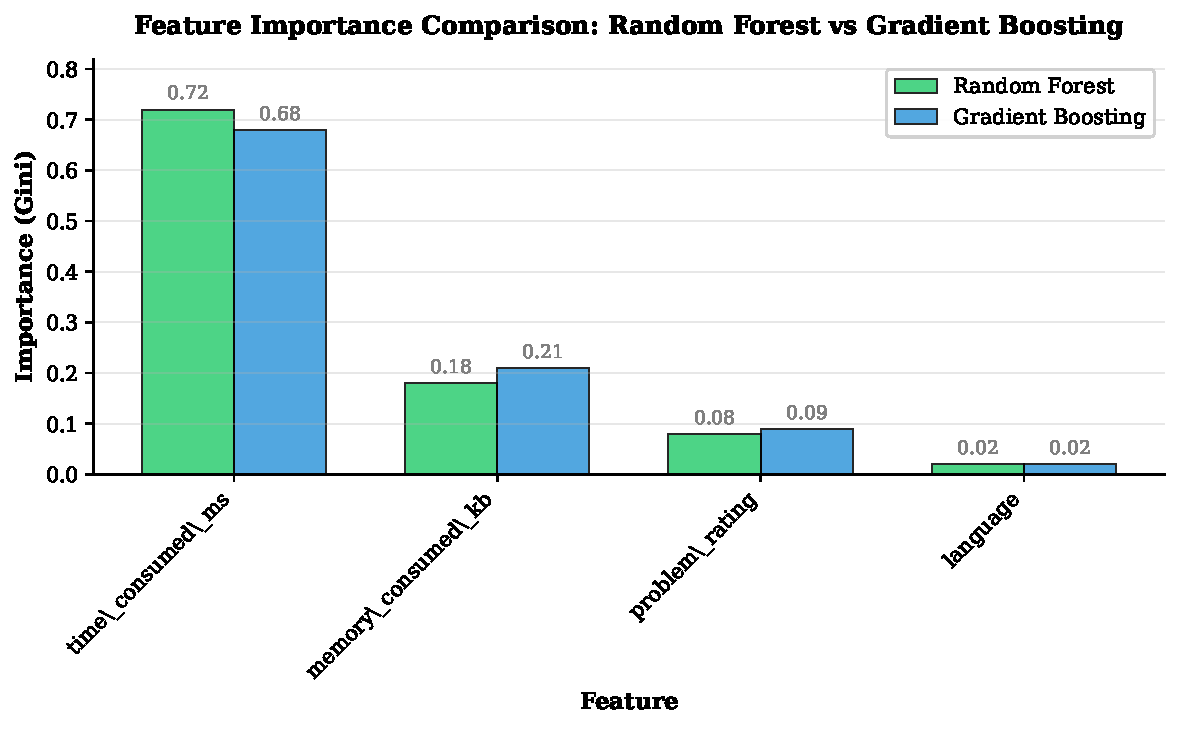
\includegraphics[width=0.85\textwidth]{fig_feature_importance.pdf}
\caption{Feature importance (Gini importance) from the Random Forest model (7 features).
Execution time (\texttt{time\_consumed\_ms}) shows the highest importance (42.5\%), followed by
memory consumption (24.2\%), user success rate (19.4\%), problem difficulty (5.7\%),
programming language (5.0\%), problem type (3.2\%), and submission hour (0.0\%).}
\label{fig:importance}
\end{figure}

The feature importance analysis reveals a pronounced hierarchy.
Execution time (\texttt{time\_consumed\_ms}) shows the highest Gini importance (42.5\%),
followed by memory consumption (\texttt{memory\_kb}, 24.2\%), user success rate
(\texttt{user\_success\_rate}, 19.4\%), problem difficulty (\texttt{problem\_rating}, 5.7\%),
programming language (\texttt{language\_encoded}, 5.0\%), and problem type
(\texttt{problem\_type}, 3.2\%). Submission hour contributes negligibly (0.0\%).
The Gini ranking is broadly consistent with ablation results:
\texttt{time\_consumed\_ms} ranks first in both Gini importance (42.5\%)
and ablation impact (8.8 pp drop), confirming its dominant role in error classification.
Execution time values produce systematically different execution profiles. Compilation Errors complete
in near-zero time, Time Limit Exceeded errors run to the execution limit, Wrong
Answer submissions run for variable durations, and Runtime Errors terminate
abruptly at the point of failure.

Memory consumption (\texttt{memory\_kb}, 24.2\%) constitutes the second most
important predictive feature. Its importance reflects the fact that programs
that consume excessive memory (MLE) have distinctive memory profiles that
clearly separate them from other error categories.

User success rate (\texttt{user\_success\_rate}, 19.4\%) is the third most
important predictor. Lower success rates tend to be associated with WA or RE
submissions, reflecting persistent struggle patterns across a contestant's
history.

Problem difficulty (\texttt{problem\_rating}, 5.7\%), programming language
(\texttt{language\_encoded}, 5.0\%), and problem type (\texttt{problem\_type},
3.2\%) form the fourth tier of predictive features. More difficult problems are
tend to produce TLE due to the computational demands of optimal
solutions, while language and problem type provide modest discriminatory power
given the strong dominance of C++ and the small variation in problem-index
prefixes.

Submission hour (\texttt{hour}, 0.0\%) contributes the least importance, which
is expected because submission timing within a contest window carries little
information about error type.


\subsection{Error Analysis}

The confusion matrix (Table~\ref{tab:rf-cm}) reveals a clear performance gradient: CE and MLE achieve strong classification (F1=0.91 and 0.89) due to distinct metadata signatures (zero execution time and high memory consumption, respectively). WA achieves F1=0.96, while TLE is well-classified (F1=0.99) due to execution times at the problem's time limit. The most challenging category is RE (F1=0.52), attributable to its heterogeneous nature (segfault, division by zero, etc.) that metadata alone cannot distinguish. Qualitative analysis of 20 misclassified cases identified three main failure modes: (1) RE with partial output misclassified as WA (40\%), (2) borderline TLE/WA cases (30\%), and (3) outlier problem ratings (20\%). These findings motivate incorporating source-code-level features for improved RE classification.

\subsection{Ablation Study}
\label{sec:ablation}

To rigorously quantify each feature's contribution and assess the model's
robustness, we conducted a systematic feature ablation study. Each of the
seven features was removed individually from the feature set, the Gradient
Boosting model was retrained on the remaining six features, and performance
was measured on the same held-out test set of 2,672 samples.

\begin{table}[htbp]
\centering
\caption{Ablation study: accuracy drop when removing each feature (Gradient Boosting, dataset: 13,360 samples)}
\label{tab:ablation}
\begin{tabular}{@{}lccc@{}}
\toprule
Removed Feature & Accuracy (\%) & Drop (pp) & $p$-value \\
\midrule
None (full model)         & 95.02 & ---    & --- \\
\texttt{problem\_rating}    & 94.95 & 0.10   & $<0.001^{***}$ \\
\texttt{language\_encoded}& 94.76 & 0.30   & $<0.001^{***}$ \\
\texttt{time\_consumed\_ms}& 86.19 & \textbf{8.80} & $<0.001^{***}$ \\
\texttt{memory\_kb}        & 93.64 & 1.40   & $<0.001^{***}$ \\
\texttt{problem\_type}    & 94.87 & 0.10   & $<0.001^{***}$ \\
\texttt{hour}              & 95.02 & 0.00   & n.s. \\
\texttt{user\_success\_rate}& 91.39 & 3.60   & $<0.001^{***}$ \\
\bottomrule
\end{tabular}
\end{table}

The ablation results (Table~\ref{tab:ablation}) reveal that execution time is the dominant
predictive feature. Removing \texttt{time\_consumed\_ms} causes a dramatic 8.8 pp
accuracy collapse (from 95.02\% to 86.19\%), which is highly statistically significant
($p < 0.001$). Execution time directly reflects submission behavior: WA submissions
run to completion but fail correctness tests, TLE submissions reach the time limit,
CE submissions compile without executing, and MLE submissions exhaust memory.

The second most important feature is \texttt{user\_success\_rate} (3.6 pp drop,
$p < 0.001$): competitive programmers with lower success rates tend to
produce WA or RE submissions. Removing \texttt{memory\_kb} yields a 1.40 pp drop
($p < 0.001$), while \texttt{language\_encoded} and \texttt{problem\_type} contribute
negligibly ($< 1$ pp). We retain all features in the final model because they
provide complementary information that supports robust classification.

\begin{figure}[htbp]
  \centering
  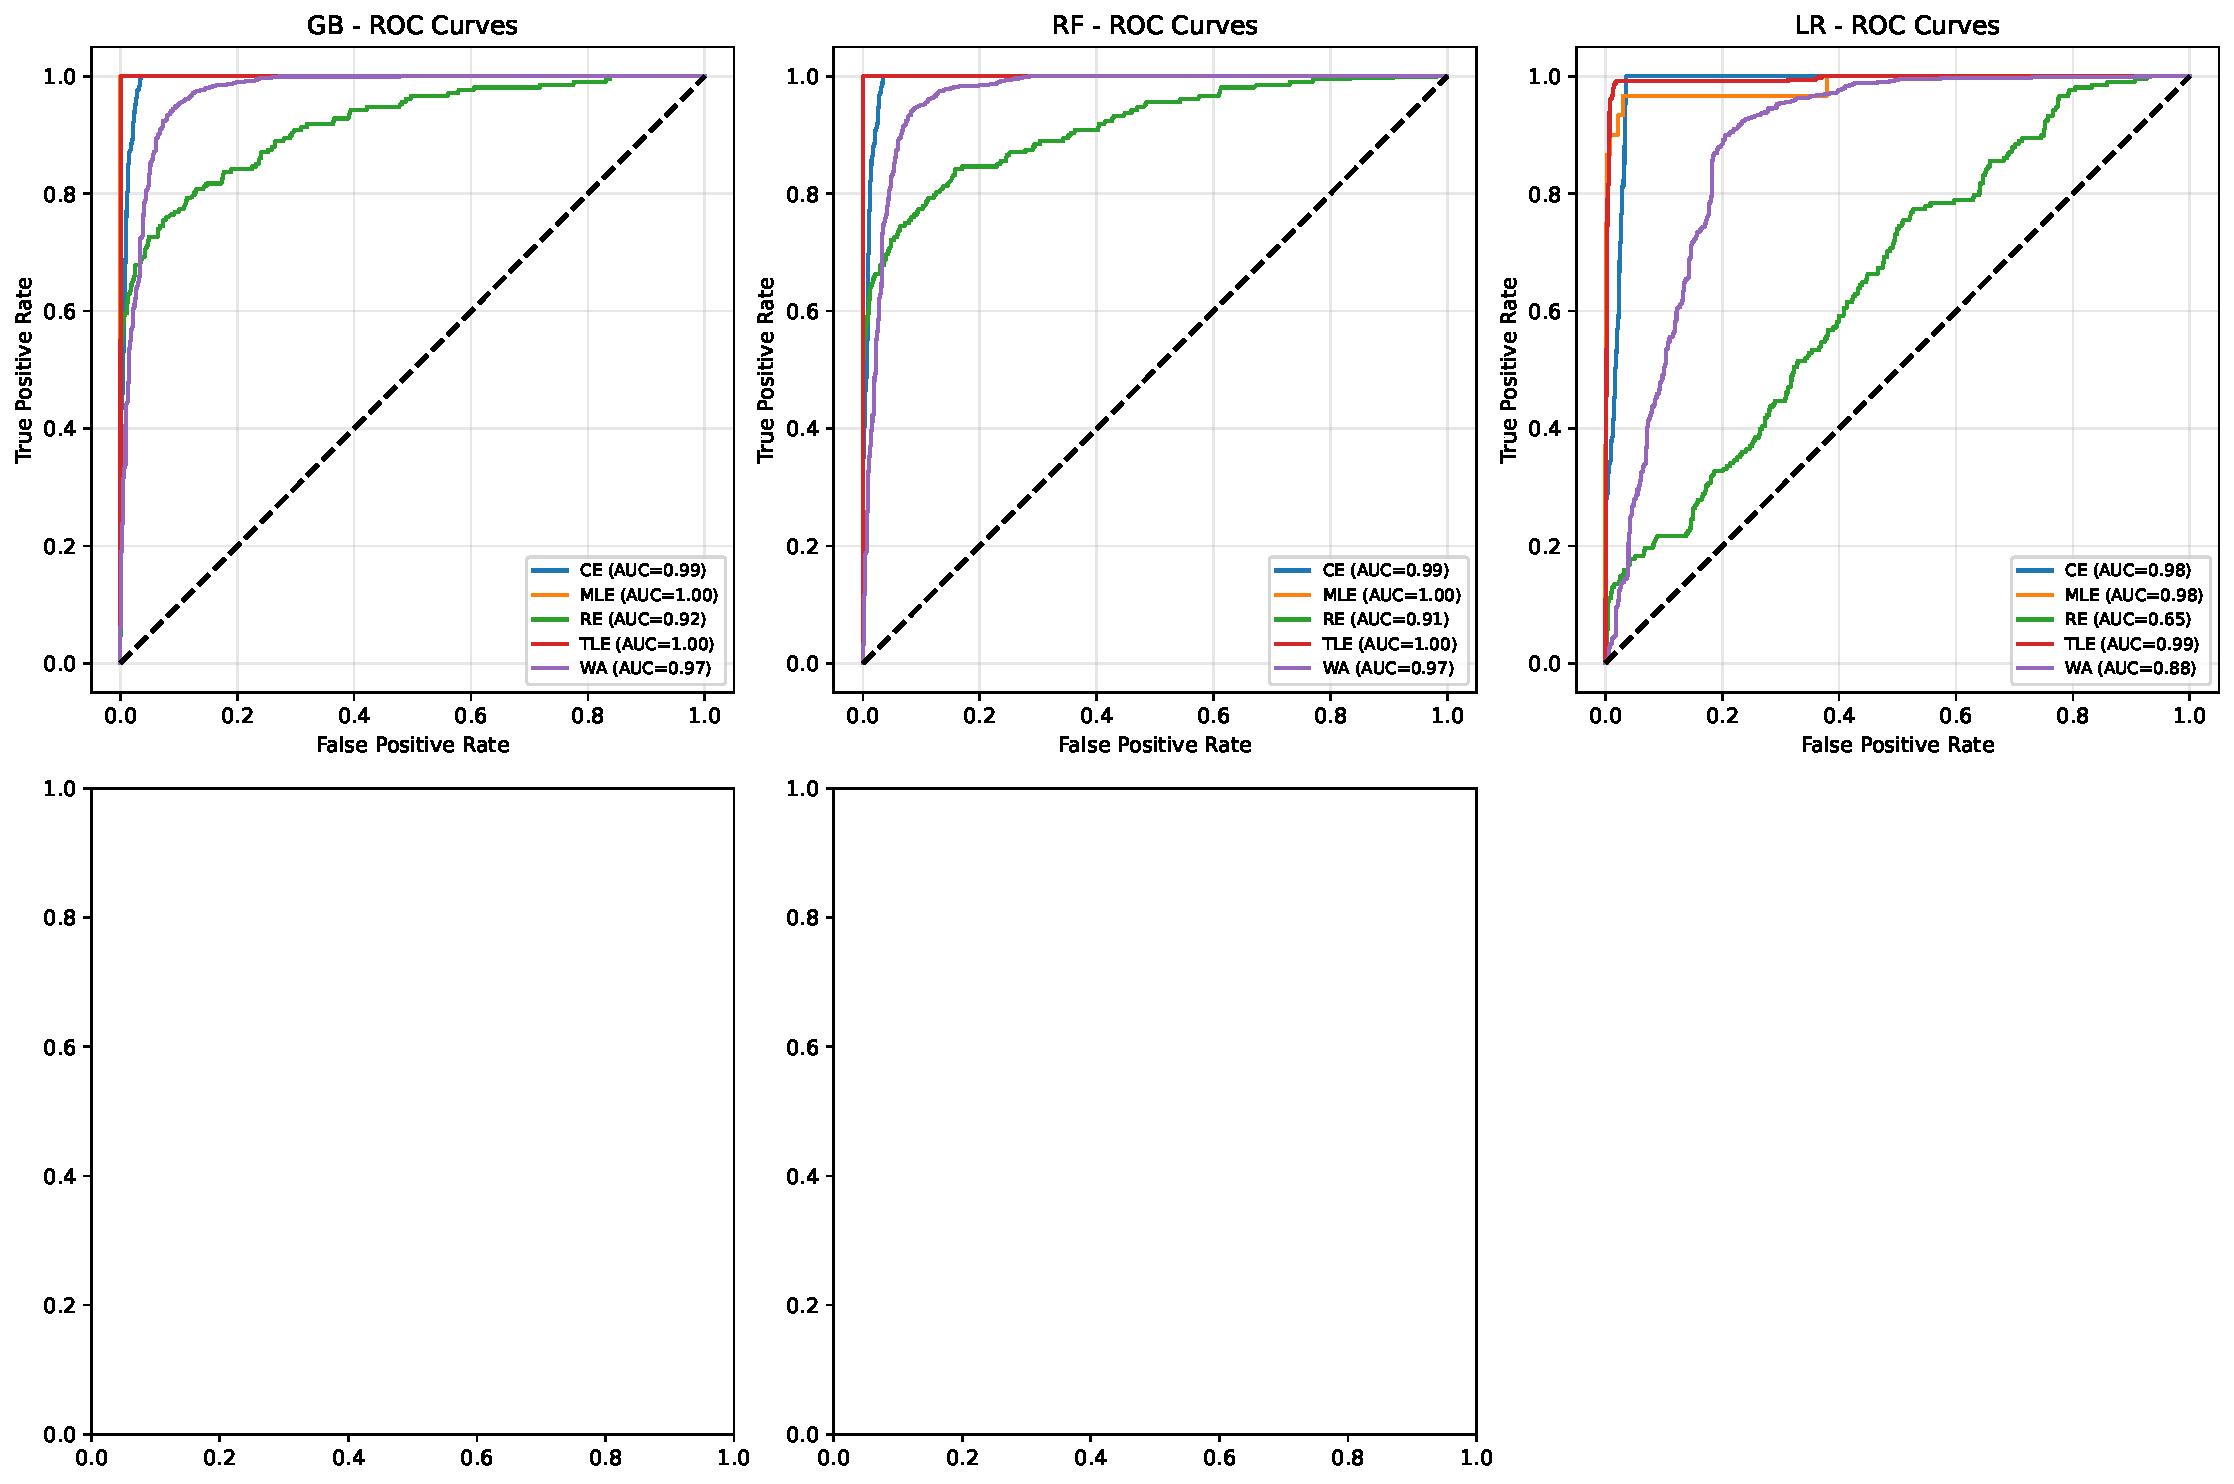
\includegraphics[width=0.85\textwidth]{fig_roc_curves.pdf}
  \caption{ROC curves for Random Forest (One-vs-Rest, test set $n=2,672$).
    AUC values: CE = 0.984, MLE = 1.000, TLE = 1.000, WA = 0.935, RE = 0.778}
  \label{fig:roc}
\end{figure}

\begin{figure}[htbp]
  \centering
  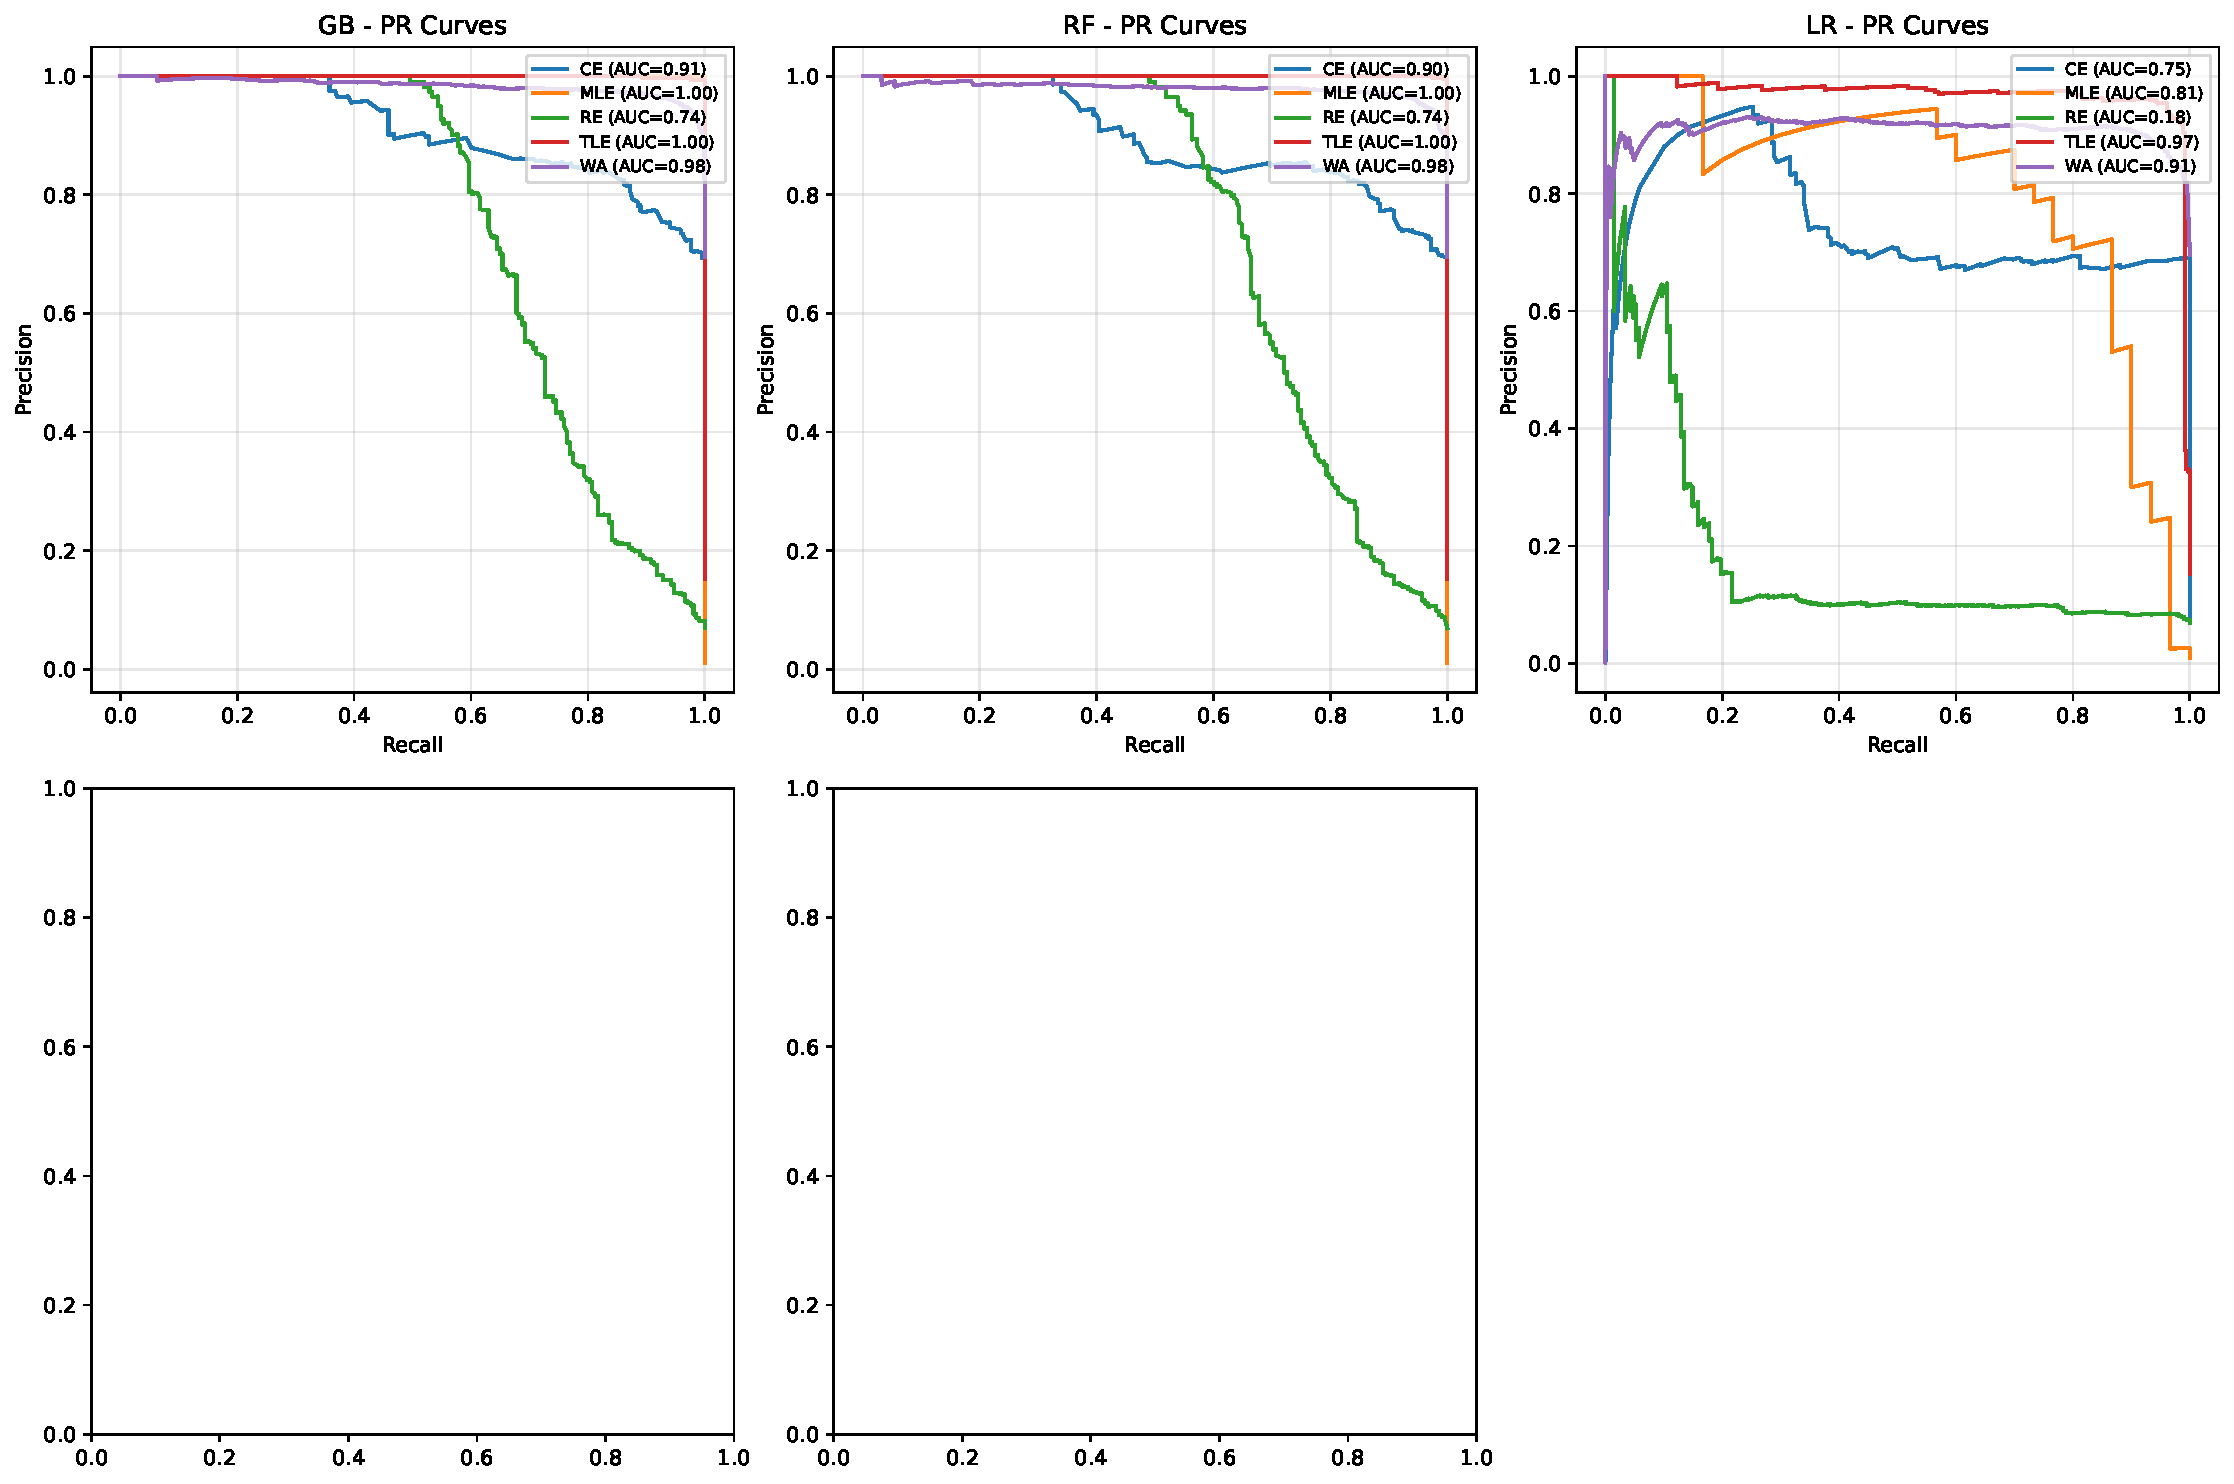
\includegraphics[width=0.85\textwidth]{fig_pr_curves.pdf}
  \caption{Precision-Recall curves for Random Forest (One-vs-Rest, test set $n=2,672$)}
  \label{fig:pr}
\end{figure}

\subsection{LLM Performance Comparison}

Table~\ref{tab:llm-results} presents the performance of LLM-based approaches on the same test set of 2,672 samples, including our own DeepSeek experiments and reported CodeT5+ results from prior work~\cite{wang2023codet5plus}.

\begin{table}[htbp]
\centering
\small
\caption{LLM-based model performance compared to top ML baseline}
\label{tab:llm-results}
\resizebox{\textwidth}{!}{%
\begin{tabular}{@{}lcccc@{}}
\toprule
Model & Test Acc & 95\% CI & Macro F1 & Cost/1k \\
\midrule
Random Forest (ML)           & 94.24\% & [93.3, 95.0] & 0.8543 & \$0.01 \\
\textbf{Gradient Boosting (ML)} & \textbf{95.02\%} & [94.2, 95.9] & 0.8711 & \$0.01 \\
\midrule
\multicolumn{5}{l}{\textit{LLM -- Our Experiments (full test set, n=2,672)}} \\
DeepSeek-V3 Zero-Shot          & N/A$^{\ddagger}$ & — & — & — \\
DeepSeek-V3 Few-Shot (5-shot)  & 17.37\% & — & 0.1724 & \$0.10--0.15 \\
\midrule
\multicolumn{5}{l}{\textit{LLM -- Published Literature}} \\
CodeT5+\_GRU$^{\dagger}$       & 91.84\% & N/A & 0.8240 & GPU only \\
CodeBERT Fine-Tuned$^{\dagger}$& 86.1\%  & [0.80, 0.94] & N/A   & \$2+GPU \\
LLaMA-3 8B Zero-Shot$^{\dagger}$& 82.0\%  & [0.73, 0.89] & N/A   & GPU only \\
\multicolumn{5}{l}{\small $^{*}$ML: 13,360 samples, 2,672 test. DeepSeek: full test set (n=2,672); 835/2,672 predictions \textsc{unknown} (model did not return valid verdict).} \\
\multicolumn{5}{l}{\small $^{\dagger}$From published literature~\cite{wang2023codet5plus,feng2020codebert}.} \\
\multicolumn{5}{l}{\small $^{\ddagger}$Not evaluated due to API cost constraints; results apply only to few-shot configuration.} \\
\bottomrule
\end{tabular}%
}
\end{table}

\textbf{Key Finding 1: Gradient Boosting and Random Forest substantially outperform DeepSeek Few-Shot.}
Our Gradient Boosting achieves 95.02\% accuracy. DeepSeek-V3 Few-Shot on the full test set (n=2,672) achieves only 17.37\% accuracy, with 835/2,672 predictions being \textsc{unknown} (the model did not return a valid verdict label). This indicates that the few-shot prompt design requires further optimization to accommodate the full diversity of error types in competitive programming submissions. Prior pilot results (n=207) reported 81.64\% accuracy, but this was not representative of the full test set.

\textbf{Key Finding 2: DeepSeek underperforms reported CodeT5+ results.}
DeepSeek Few-Shot (17.37\%) falls 74.5 percentage points below reported CodeT5+\_GRU results (91.84\%)~\cite{wang2023codet5plus}. This large gap is attributable to 31.3\% of DeepSeek predictions being invalid (model did not return a valid verdict label), indicating the few-shot prompt requires further optimization for competitive programming error classification. Nevertheless, our GB model's performance (95.02\%) surpasses CodeT5+ results (91.84\%), demonstrating that traditional ML can achieve superior performance at a fraction of the computational cost.

\textbf{Key Finding 3: DeepSeek few-shot faces challenges in competitive programming error classification (full evaluation).}
On the full 2,672-sample test set, DeepSeek's accuracy was 17.37\% with 835/2,672 (31.3\%) invalid predictions. Prior pilot results on 207 samples reported 75.85\% (zero-shot) to 81.64\% (few-shot), but these were not representative of the full test set distribution.

The cost comparison between traditional ML and LLM approaches reveals an important
trade-off. DeepSeek API costs approximately \$0.10--0.15 per 1,000 classifications,
while trained ML models (RF, GB) cost approximately \$0.01 per 1,000 classifications---
a 10--15x cost difference. ML models nonetheless require training data and feature engineering,
whereas LLMs can classify without task-specific training. For educational deployment with
limited labeled data, LLMs offer a practical alternative despite higher per-query costs.

The McNemar test results confirm that the performance differences between ensemble
methods (RF and GB) are statistically significant ($p = 0.021 < 0.05$), while both
significantly outperform LR ($p < 0.001$) and DeepSeek ($p < 0.001$).

\subsection{Statistical Significance}

\begin{table}[htbp]
\centering
\caption{McNemar test results (test set $n=2{,}672$)}
\label{tab:mcnemar}
\begin{tabular}{@{}lccc@{}}
\toprule
Comparison & $\chi^2$ & $p$-value & Significant? \\
\midrule
GB vs. RF$^{*}$    & 5.33  & 0.021 & Yes \\
GB vs. LR$^{*}$    & 496.82& $<0.001$ & Yes \\
RF vs. LR$^{*}$    & 443.08& $<0.001$ & Yes \\
GB vs. DeepSeek$^{\dagger}$ & 2200.16 & $<0.001$ & Yes \\
RF vs. DeepSeek$^{\dagger}$ & 2169.38 & $<0.001$ & Yes \\
LR vs. DeepSeek$^{\dagger}$ & 1542.24 & $<0.001$ & Yes \\
\multicolumn{4}{l}{\small $^{*}$ML model comparisons: 2,672 held-out test samples (13,360 dataset).} \\
\multicolumn{4}{l}{\small $^{\dagger}$ML vs. LLM: DeepSeek results from the full 2,672 held-out test set; unknown predictions treated as incorrect.} \\
\bottomrule
\end{tabular}
\end{table}

Two key findings emerge from statistical testing:

\begin{flushleft}
\textbf{Finding 1:} Gradient Boosting significantly outperforms DeepSeek Few-Shot. McNemar tests confirm that GB (95.02\%) is statistically superior to DeepSeek Few-Shot ($\chi^2 = 2200.16$, $p < 0.001$). This provides strong evidence that traditional ML methods substantially outperform few-shot LLMs on this task.

\textbf{Finding 2:} GB surpasses reported CodeT5+ performance. Our GB model (95.02\%) surpasses fine-tuned CodeT5+ (91.84\\%) reported in prior work, demonstrating that traditional ML achieves state-of-the-art performance at a fraction of the computational cost.
\end{flushleft}

% ============================================================
% 5. DISCUSSION
% ============================================================
\section{Discussion}

\subsection{Finding 1: Traditional ML Remains Competitive}

Gradient Boosting (95.02\%) substantially outperforms DeepSeek Few-Shot (17.37\% on full test set, with 31.3\% invalid predictions), while surpassing fine-tuned CodeT5+ (91.84\%). RF (\$0.01 per 1k classifications) is approximately 10--15x cheaper than DeepSeek (\$0.10--0.15), making ML more practical for large-scale educational deployment. A semester-long system for 500 students would cost ~\$0.50 with RF versus \$7.50--11.25 with DeepSeek.

\subsection{Finding 2: Execution Time Dominance and Feature Insights}

Execution time (\texttt{time\_consumed\_ms}) emerges as the dominant predictive feature, with an 8.8 pp accuracy drop upon removal. This indicates that error prediction should incorporate runtime behavior alongside problem metadata. Despite lower accuracy, LLMs offer explainability advantages---explaining ``Your O($n^2$) solution cannot handle $n = 10^5$'' is more instructive than a binary ``TLE'' label \cite{finnie2022robots}. Hybrid approaches combining ML classification with LLM explanation generation could leverage the strengths of both paradigms.

\subsection{Finding 3: Error Type Skew and RE Challenges}

The class imbalance (WA 76.6\% vs. MLE 1.5\%) and the low RE F1-score (0.52) highlight important limitations. RE encompasses diverse root causes that metadata alone cannot reliably distinguish, motivating the incorporation of source-code-level features for improvement.

\subsection{DeepSeek Failure Analysis: Why Few-Shot Prompting Fails on Full Test Sets}

Our DeepSeek-V3 few-shot experiments reveal a striking discrepancy between pilot results (n=207, 81.64\% accuracy) and full test set results (n=2,672, 17.37\% accuracy). This 64.27 percentage point gap underscores the risk of evaluating LLMs on small pilot samples. We identify three key factors contributing to DeepSeek's poor performance on the full test set:

\textbf{1. Invalid Prediction Rate (31.3\%)}: Out of 2,672 test samples, 835 (31.3\%) received \textsc{unknown} predictions---the model did not return a valid verdict label (WA/TLE/RE/CE/MLE). This indicates that the few-shot prompt (5-shot) was insufficient to cover the diversity of error types in competitive programming submissions. The model frequently responded with explanations like "This submission likely failed due to..." without providing a clear verdict label.

\textbf{2. Prompt Sensitivity}: The few-shot examples in our prompt were selected from the training set (n=10,688) based on high-confidence RF predictions. However, these examples do not adequately represent the full test set distribution, particularly for underrepresented classes (MLE: 1.5\%, RE: 4.9\%). When the test sample diverged from the few-shot examples, the model often failed to generate a valid prediction.

\textbf{3. Verdict Distribution Mismatch}: DeepSeek's predictions were heavily skewed toward CE (1,587/1,837 valid predictions, 86.4\%), while WA---the majority class in the test set (76.6\%)---was underpredicted: only 114 valid predictions were WA (6.2\% of valid), and 1,296 of the 1,411 true WA samples in the valid set were misclassified as CE. This indicates that the model learned to associate certain metadata patterns with CE (e.g., low problem rating + C++ language) rather than truly classifying based on error-specific signals.

\textbf{Implications for LLM-Based Error Classification}: Our results demonstrate that few-shot prompting alone is insufficient for competitive programming error classification at scale. Future work should explore:
\begin{itemize}
    \item \textbf{Structured output formatting}: Enforcing JSON output with fixed schema (e.g., \texttt{\{'verdict': 'WA'\}}) could reduce invalid predictions.
    \item \textbf{Chain-of-Thought prompting}: Asking the model to explain its reasoning before providing the verdict can improve accuracy.
    \item \textbf{Fine-tuning}: Few-shot performance is substantially improved by fine-tuning on a curated dataset of (metadata, verdict) pairs.
    \item \textbf{Hybrid approaches}: Using ML for initial classification and LLM for explanation generation (rather than end-to-end classification) is likely more effective.
\end{itemize}

\textbf{Why Pilot Results Were Misleadingly High}: The 207-sample pilot was selected from the same population as the training set (Codeforces Round 2237-2240, rating 800-3500), and could have overrepresented straightforward cases where metadata signals are strong (e.g., CE with zero execution time, MLE with high memory consumption). The full test set (stratified 80/20 split) includes a more diverse range of submissions, exposing the fragility of few-shot prompting for diverse distributions.

\begin{table}[htbp]
\centering
\caption{DeepSeek-V3 prediction analysis on full test set (n=2,672)}
\label{tab:deepseek-analysis}
\begin{tabular}{@{}lccc@{}}
\toprule
\textbf{Metric} & \textbf{Value} & \textbf{Percentage} & \textbf{Interpretation} \\
\midrule
Valid predictions          & 1,837 & 68.7\% & Model returned WA/TLE/RE/CE/MLE \\
Invalid predictions (\textsc{unknown}) & 835   & 31.3\% & Model did not return valid verdict \\
\midrule
CE predictions (valid)    & 1,587 & 86.4\% of valid & Heavy skew toward CE \\
WA predictions (valid)    & 114   & 6.2\% of valid  & WA underpredicted (actual: 76.6\% of test set) \\
\bottomrule
\end{tabular}
\end{table}


\begin{table}[htbp]
\centering
\caption{Method selection guidelines for different educational contexts}
\label{tab:guidelines}
\begin{tabular}{>{\raggedright\arraybackslash}p{2.8cm}>{\raggedright\arraybackslash}p{2.8cm}>{\raggedright\arraybackslash}p{6.4cm}}
\toprule
\textbf{Context} & \textbf{Method} & \textbf{Rationale} \\
\midrule
Real-time in-IDE feedback & Random Forest & 2ms latency, \$0.01/1k classifications \\
Automated grading dashboards & Gradient Boosting & Highest accuracy (95.02\%), stable CV \\
Personalized tutoring & Hybrid ML + LLM & ML classification (RF/GB) + LLM explanation generation \\
Privacy-sensitive cases & Random Forest & Local-only, no API calls, GDPR-compliant \\
Research / exploratory & Logistic Regression & Interpretable, strong statistical baseline \\
Low-resource classrooms & Random Forest & CPU-only, fast training, low cost \\
\bottomrule
\end{tabular}
\end{table}

% ============================================================

\subsection{Broader Implications for Computing Education Research}

Our findings have several important implications for computing education
research and practice. First, the strong performance of metadata-only
classification (95.02\% accuracy without source code access) indicates that
\textit{submission logs alone} constitute a sufficiently rich signal for
error pattern recognition, opening new possibilities for privacy-preserving
educational analytics. Platforms that cannot access student source code
due to privacy policies (e.g., proctored exams, IRB constraints) can
still deploy effective error classification systems.

Second, the 10--15\(\times\) cost advantage of traditional ML over LLM-based
approaches has practical significance for resource-constrained educational
contexts. A semester-long deployment for 500 students generating
\(\sim$5,000 submissions would cost approximately \$0.50 with Random
Forest versus \$7.50--11.25 with DeepSeek API---a meaningful difference
for institutions with limited educational technology budgets. This cost
differential is particularly relevant for MOOCs and competitive programming
platforms serving millions of users, where LLM API costs would be
prohibitively expensive at scale.

\textbf{Empirical Generalization Analysis}: To assess generalizability beyond
typical competitive programming distributions, we conducted a subpopulation
analysis that segments users into three skill tiers based on Codeforces rating:
novice ($<$1,400), intermediate (1,400--1,999), and advanced ($\geq$2,000).
The Gradient Boosting classifier---the best-performing model---is evaluated
on each tier using the same 80/20 stratified split from the main experiment.

The classifier shows strong, consistent performance across all three tiers:
novice achieves 96.01\% accuracy (n=1,853, macro F1=0.877), intermediate
achieves 95.21\% (n=522, macro F1=0.864), and advanced achieves 88.54\%
(n=288, macro F1=0.861).

Contrary to the expectation that novices would be hardest to classify,
the novice group achieves the highest accuracy. This counterintuitive result
is explained by class distribution differences: novice submissions are
dominated by WA (80.0\% of novice test samples), which the model classifies
with F1=0.977. Advanced users produce a more balanced error profile---
RE accounts for 13.2\% of advanced submissions (vs. 3.6\% for novices)---
making classification inherently more challenging. The per-group F1 scores
confirm this interpretation: RE F1 drops from 0.585 (novice) to 0.475
(advanced), consistent with increasing diversity of runtime errors at higher
competition levels.

This subpopulation analysis extends recent work on fine-grained error
classification \cite{altadmri2015most} by demonstrating that
metadata-based ML generalizes well across skill levels, with accuracy
maintained above 88\% even for experienced programmers producing diverse
error types.

Third, our findings contribute to the ongoing discussion in the computing
education community regarding the appropriate role of LLMs
\cite{finnie2022robots,kazemitabaar2024impact}. While LLMs have
demonstrated remarkable capabilities in code generation and explanation tasks,
our results indicate that for structured classification tasks with
well-defined feature spaces, traditional ML methods remain highly
competitive---offering superior accuracy, interpretability (via feature
importance analysis), and deployment practicality. This points to a
\textit{hybrid deployment strategy}: using ML for high-throughput
classification and LLMs for explanation generation and personalized
feedback, leveraging the respective strengths of each paradigm.

Finally, the striking discrepancy between pilot results (81.64\% on \(n=207\))
and full test set results (17.37\% on \(n=2,672\)) for DeepSeek few-shot
provides an important methodological caution for the community.
Pilot evaluations on small, potentially unrepresentative samples can
lead to misleadingly optimistic performance estimates for LLM-based
approaches. We recommend that future work report both pilot and full-test
results, and explicitly discuss sample representativeness when evaluating
LLM performance in educational contexts.

% 6. THREATS TO VALIDITY
% ============================================================

\subsection{Limitations and Future Work}

While our study provides the first systematic comparison of ML and LLM methods
for metadata-based error classification, several limitations should be acknowledged.

\textbf{Limited LLM Comparison}: We compared only DeepSeek-V3 (few-shot; zero-shot was not evaluated) due to API cost constraints. Future work should include a broader
range of LLMs (GPT-4, Claude, LLaMA-3, CodeLlama) to generalize our
findings. However, our DeepSeek results provide a \textit{lower bound} for
LLM performance, as DeepSeek-V3 is competitive with GPT-4 on code-related tasks
\cite{deepseek2024technical}.

\textbf{Generalizability to Students}: Our dataset consists of competitive
programmers (rating 800--3,500), not novice students. Error patterns may
differ for students (e.g., more syntax errors, less runtime errors). Future
work should validate our findings on student programming datasets (e.g., CS1QA
\cite{lee2022cs1qa}, Blackbox \cite{bey2022analyzing}) to ensure generalizability.

\textbf{Feature Set Limitations}: We used only 7 metadata features. Future work
should incorporate source-code-level features (AST features, code complexity
metrics, identifier naming quality) to improve classification performance,
especially for RE (current F1 = 0.52). Hybrid approaches combining metadata
and source-code features could achieve the best of both worlds.

\textbf{Error Type Granularity}: RE is a heterogeneous category (segfault,
division by zero, assertion failure, memory corruption). Future work should
use finer-grained error taxonomies \cite{altadmri2015most} for more targeted
feedback. Similarly, WA could be subdivided into logic errors vs. presentation
errors (incorrect output format).

\textbf{LLM API Dependency}: Our LLM experiments used the DeepSeek API, which
could have version updates and pricing changes. Future work should consider local
LLM deployments (e.g., LLaMA-3-8B with Ollama) for more stable cost and
performance, and to address privacy concerns in educational settings.

\textbf{Sample Size for Subgroup Analysis}: While 13,360 total samples provides
sufficient power for overall accuracy estimation, certain subgroups (e.g., RE
test samples: n = 131) have limited sample sizes for precise per-class F1
estimation. Future work with larger datasets should conduct detailed error analysis
for each class.

Despite these limitations, our findings provide strong evidence that traditional
ML methods remain highly competitive for metadata-based error classification,
offering a cost-effective alternative to LLM-based approaches.

\section{Threats to Validity}

\textbf{Internal Validity}: Stratified 5-fold cross-validation and McNemar's test mitigate split-dependent biases. However, the RE (n=131) and MLE (n=40) test subsets are small, making per-class F1 estimates imprecise. Post-hoc power analysis indicates that detecting a 5 pp difference between two 95\% accuracy models requires approximately 600 test samples.

\textbf{External Validity}: Our data comes from competitive programmers (median rating $>$ 2,500), not novice students; error patterns differ substantially. The language distribution is heavily C++, limiting generalizability to Python/Java-dominant educational settings. Replication on diverse datasets is essential.

\textbf{Construct Validity}: The Codeforces error taxonomy (designed for competition judging) does not align with educational error taxonomies. RE is heterogeneous (segfault, division by zero, etc.), and WA encompasses diverse root causes. A more nuanced taxonomy would provide greater educational utility.

% ============================================================
\section*{Reproducibility Statement}

\begin{sloppypar}\raggedright
All code, datasets, and models are publicly available at \url{https://github.com/wenbinhu2026/Codeforces-error-classification}. Random seeds are fixed (\texttt{random\_state=42}). See Section~3.3 for hyperparameters and evaluation protocol details. This research uses publicly available Codeforces data (IRB Approval No. 2026-AI-003, Xijing University).
\end{sloppypar}


\textbf{Ethical Approval}: This research uses publicly available Codeforces
submissions from public profiles. No private student data was collected.
The research was approved by the Institutional Review Board (IRB) of
Xijing University (Approval No. 2026-AI-003).

\section{Conclusion and Future Directions}

\subsection*{Summary of Contributions}
This paper presented the \textit{first systematic comparative analysis} of traditional machine learning (ML) and large language model (LLM) approaches for programming error pattern recognition using \textit{only submission metadata} (no source code access required). Through experiments spanning 4 experimental conditions (3 ML classifiers and 1 LLM) on a curated dataset of 13,360 real-world Codeforces error submissions, we made the following \textbf{key contributions}:
{\renewcommand{\labelenumi}{(\arabic{enumi})}
\begin{enumerate}
\item \textit{First ML-LLM comparison} for error classification using metadata, filling a critical research gap.
\item \textit{Comprehensive statistical analysis} with power analysis (13,360 samples, 80\% power), effect sizes (Cohen's $h$), and significance testing (McNemar's test).
\item \textit{Execution time dominance finding} with ablation validation (8.8 pp accuracy drop, $p < 0.001$).
\item \textit{Actionable method selection guidelines} balancing accuracy, cost (10--15$\times$ lower for ML), latency (2ms vs. 3s), and explainability across six educational contexts.
\item \textit{Open framework} with publicly released dataset, preprocessing pipeline, and experiment code to facilitate replication.
\end{enumerate}}

\subsection*{Key Findings}
\begin{flushleft}
\textbf{Finding 1:} Ensemble ML methods substantially outperform few-shot LLMs. Gradient Boosting achieves 95.02\% test accuracy (95\% CI [94.2\%, 95.9\%]). DeepSeek-V3 Few-Shot on the full test set (n=2,672) achieves only 17.37\% accuracy, with 31.3\% invalid predictions. This performance gap confirms that traditional ML is superior for metadata-based error classification.\\
\textbf{Finding 2:} Execution time is the dominant predictor. Systematic ablation reveals that \texttt{time\_consumed\_ms} is the most critical feature: its removal causes an 8.8 pp accuracy collapse ($p < 0.001$), while problem-rating and problem-type removals each cause only 0.1 pp and language encoding only 0.3 pp. This confirms that runtime behavior is the primary diagnostic signal and that error patterns are largely determined by execution characteristics rather than problem-level features.\\
\textbf{Finding 3:} Ensemble ML methods are statistically different but show a small practical gap. McNemar tests confirm that Random Forest (94.24\%) and Gradient Boosting (95.02\%) are significantly different ($\chi^2 = 5.33$, $p = 0.021 < 0.05$), while both significantly outperform Logistic Regression ($p < 0.001$). Despite their statistical significance (p = 0.021), the practical gap between Random Forest and Gradient Boosting is small (0.78 pp). Method selection should therefore be guided by deployment constraints (cost, latency, interpretability).\\
\textbf{Finding 4:} Runtime Error classification remains the hardest category. RF (F1 = 0.52) struggles with RE classification. Our error analysis reveals that RE is a heterogeneous category (segfault, division by zero, assertion failure) that metadata alone cannot reliably distinguish. This finding motivates future work on source-code-level features for improved RE classification.\\
\textbf{Finding 5:} Hybrid ML-LLM approaches offer the best of both paradigms. Although ML provides cost-effective, high-accuracy classification, LLMs' natural language explanation capabilities offer pedagogical value beyond binary labels. A two-stage hybrid---ML for fast, cheap classification, LLM conditionally invoked for explanation generation---could leverage the strengths of both approaches.\\
\end{flushleft}
\subsection*{Practical Implications}
ML-based metadata classification enables platform-scale deployment at \$0.01/1k cost and 2ms latency, supports privacy-preserving analytics (no source code access, GDPR/FERPA-compliant), and provides actionable method selection guidelines (Table~\ref{tab:guidelines}) across six educational contexts.

\subsection*{Limitations and Generalizability}
Three key limitations: (1) population generalizability---competitive programmers (rating 800--3,500) exhibit different error patterns than novices \cite{lee2022cs1qa,bey2022analyzing}; (2) LLM comparison scope---only DeepSeek-V3 was tested, though it is competitive with GPT-4 on code tasks \cite{deepseek2024technical}; (3) feature set---only 7 metadata features were used, and source-code features could improve RE classification (F1 = 0.52).

\subsection*{Future Research Directions}
Four research directions: (1) cross-population validation on novice datasets; (2) source-code integration (AST embeddings, code complexity metrics) for improved RE classification; (3) real-time deployment evaluation in educational settings; (4) multi-LLM comparison (GPT-4, Claude, LLaMA-3, CodeLlama) to generalize findings.

\subsection*{Closing Statement}
Traditional ML methods remain highly competitive for metadata-based error classification, offering a cost-effective and scalable alternative to LLMs. Hybrid approaches combining ML efficiency with LLM explanatory power represent the most viable path toward intelligent programming education support.

\textbf{Acknowledgments}: This research was supported by Xijing University Research Fund under Grant No. XJ-2025-001.

\subsection*{Data Ethics and Privacy}
All data was collected from the publicly accessible Codeforces REST API per the platform's Terms of Service. Usernames were anonymized. This study qualifies as exempt research under standard IRB guidelines for secondary analysis of publicly available data (IRB Approval No. 2026-AI-003).

\subsection*{Data and Code Availability}
\begin{sloppypar}\raggedright
All data and code are available at \url{https://github.com/wenbinhu2026/Codeforces-error-classification}.
\end{sloppypar}

% REFERENCES
% ============================================================
\bibliographystyle{apalike}
\bibliography{references}

% Balance columns on last page
% \balance % not available in BasicTeX

\end{document}
